\documentclass{beamer} % [notes=only]
\usetheme{Intel}

\setbeamertemplate{section in toc}{\inserttocsectionnumber.~\inserttocsection} % Use number keys for table of content sections.
\setbeamertemplate{subsection in toc}{\hspace{0.5cm}\rule[0.3ex]{3pt}{3pt}~\inserttocsubsection\par} % Use a symbol for table of content subsections.
\AtBeginSection[]
{
	\begin{frame}
		\frametitle{Table of Contents}
		\tableofcontents[currentsection]
    \end{frame}
} % Insert table of contents frame before each new section.
\setbeamertemplate{caption}[numbered] % Number figures.

\definecolor{intel}{RGB}{0, 113, 197}
\setbeamercolor{section in toc shaded}{fg=intel}
\setbeamercolor{subsection in toc shaded}{fg=black}
\setbeamercolor{section in toc}{fg=intel}
\setbeamercolor{subsection in toc}{fg=black}
\setbeamercolor{block title}{fg=intel}
\setbeamercolor{caption name}{fg=intel}

\usepackage{hyperref}
\usepackage{multicol} % Used to split up table of contents in a double column style.
\usepackage{multirow} % Needed for multirow graphs
\usepackage{datetime} % Used to format dates.
\usepackage{listings} % Used to format inline code throughout document.
\usepackage{color} % Used to gray out text
\usepackage{tikz} % Used to gain access to the \centering command.
\usepackage[mediumspace,mediumqspace,squaren,binary]{SIunits} % \milli\second
\usepackage{keystroke} % Used for key icons.

\hypersetup{
	colorlinks=false,
	linkcolor=blue,
	urlcolor=black,
	citecolor=blue,
	anchorcolor=blue
}
\usetikzlibrary{calc}

\newenvironment{graytext}{\color{gray}}{\ignorespacesafterend}

\newcommand{\mascfirstline}[1]{\input{#1}\unskip}

\lstset{
	language=C,
	tabsize=4,
	backgroundcolor=\color{black!5},
	basicstyle=\tiny,
}

\newcommand{\dvtcmdcodeinline}[1]{
	\colorbox{black!5}{
			\lstinline[basicstyle=\ttfamily\color{black}]{#1}}}

\newtheorem{thm}{Key point}

\begin{document}
	\title{Paravirtualizing OpenGL ES in Simics}
\subtitle{Master's Thesis in Computer Science}
\author{Eric Nilsson}
\institute{Intel Corporation}
\date{\today}

\begin{frame}
	\titlepage
\end{frame}


	\section{Introduction}

	\subsection{Simics}
	\begin{frame}

\frametitle{Wind River\texttrademark\ Simics\texttrademark }

\begin{itemize}
	\item Full-system simulator\note{That is; a fast and functional simulator that runs unmodified software}
	\item Originally devised at SICS\footnote{The Swedish Institute of Computer Science.}\note{This was the first instance of an unmodifed OS running in an entirely simulated environment}
	\item Developed by Intel\textregistered 
	\item Sold through Intels subsidiary Wind River Systems, Inc.
	\item Used in the industry by groups such as:
	\begin{itemize}
		\item IBM
		\item NASA
		\item Lockheed Martin
	\end{itemize}
	\item Utilized extensively in academia\footnote{$300+$ universities.}
\end{itemize}

\end{frame}


        \subsection{Terminology}
        \begin{frame}
\frametitle{Paravirtualization}

\begin{center}
  \textit{"selectively modifying virtual architecture to enhance\\
scalability, performance, or simplicity"}
\end{center}

\begin{center}
  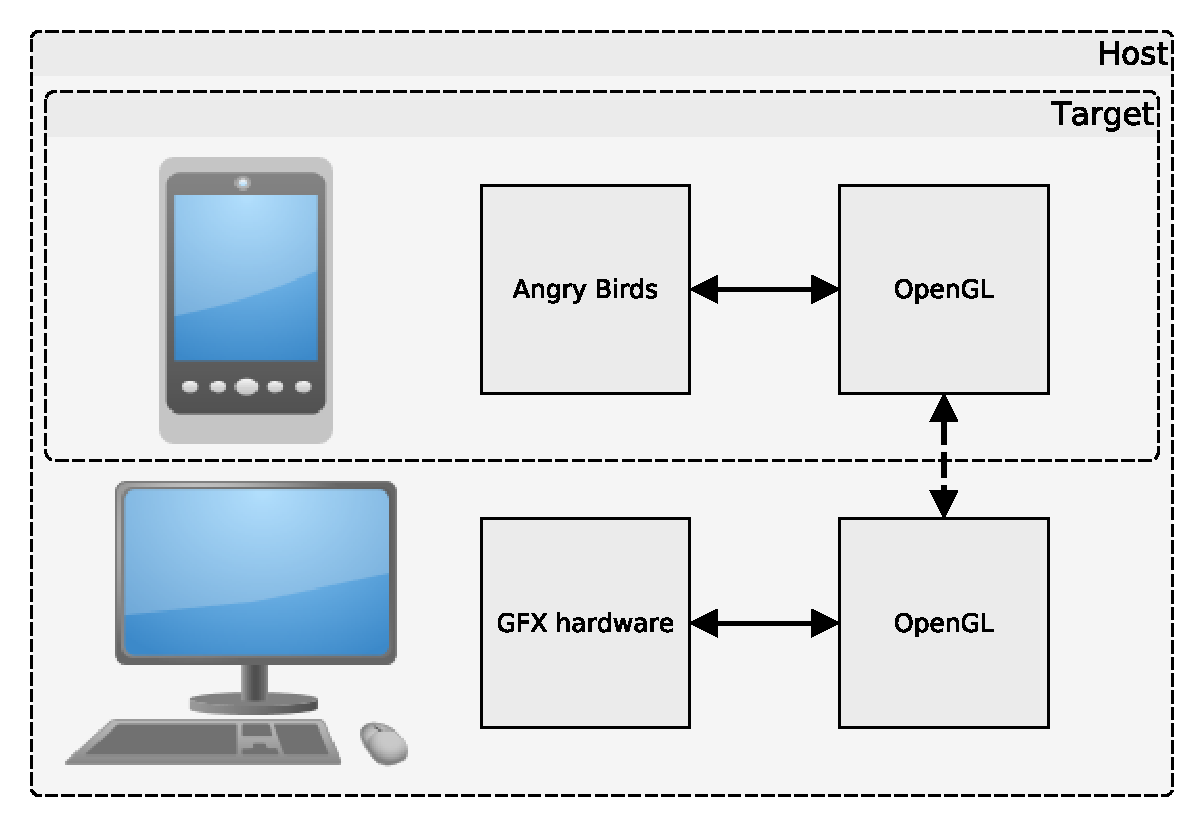
\includegraphics[height=0.7\textheight]{yedparavirtualization.pdf}
\end{center}

\end{frame}

        \begin{frame}
\frametitle{Hardware-assisted virtualization}

\begin{itemize}
\item To accelerate simulation, Simics relies on:
  \begin{itemize}
  \item Interpretation
  \item Just-in-Time compilation
  \end{itemize}
\item For Intel\circledR\ Architecture targets, Simics can utilize hardware-assisted virtualization\footnote{'accelerated virtualization', 'native virtualization'} to drastically improve performance
\end{itemize}

\end{frame}


	\subsection{Question formulation}
	\begin{frame}
\frametitle{Question formulation}

\begin{block}{\#1}
  Is paravirtualization is a viable method of accelerating graphics?
\end{block}

\begin{block}{\#2}
  Are magic instructions is a suitable communications medium?
\end{block}

\begin{block}{\#3}
  How does hardware-assisted virtualization impact graphics acceleration using paravirtualization?
\end{block}

\end{frame}


        \subsection{Background}
        \begin{frame}
\frametitle{Background}

\begin{itemize}
\item Virtual platforms are key to reducing Time-to-Market
\item Improved simulation performance enables more use-cases
\item Because of architectural differences, GPU workloads are sub-optimal for CPUs
\item Therefore, some method of accelerating graphics in Simics is desireable
\end{itemize}

\begin{center}
{\Huge $\hookleftarrow$}
\end{center}

\end{frame}

        \begin{frame}
\frametitle{User example - Tracing}

An example of why paravirtualization in Simics is of interest

\end{frame}


	\subsection{Graphics simulation}
	\begin{frame}
\frametitle{Graphics simulation}

\begin{columns}
	\column{0.5\textwidth}
	\begin{block}{GPU modeling}
		Modeling the GPU ISA
                \begin{itemize}
                  \item Costly
                  \item Performance obstacles
                \end{itemize}
	\end{block}
	\begin{block}{PCI passthrough}
		First-hand device access using passthrough technologies
                \begin{itemize}
                  \item Requires dedicated hardware\phantom{     }
                  \item Difficult to implement robust checkpointing
                \end{itemize}
	\end{block}
    \column{0.5\textwidth}
    \begin{block}{Soft modeling}
    	Software rasterization
        \begin{itemize}
        \item Easy but often good-enough
        \item Performance obstacles
        \end{itemize}
    \end{block}
    \begin{block}{Paravirtualization}
    	Selectively modify virtual architecture
        \begin{itemize}
          \item Facilitate checkpointing in software
          \item Cost-effective but possibly heavy maintenence
        \end{itemize}
    \end{block}
\end{columns}
	
\end{frame}


        \section{Methodology and experiment}

        \subsection{Summary}
	\begin{frame}
  \frametitle{Summary}

  \begin{columns}
  \column{0.5\textwidth}

  \begin{block}{Method}
    \begin{itemize}
    \item Paravirtualized graphics
    \item Accelerates OpenGL ES 2.0
    \end{itemize}
  \end{block}

  \begin{block}{Evaluation}
    \begin{itemize}
    \item Run benchmarks stressing suspected optimal and sub-optimal use-case
    \item Compare performance to software rasterization
    \end{itemize}
  \end{block}

  \begin{block}{Conclusion}
    \begin{itemize}
    \item Improved performance, $34\times$
    \item Located bottleneck
    \end{itemize}
  \end{block}

  \column{0.5\textwidth}

  \begin{center}
    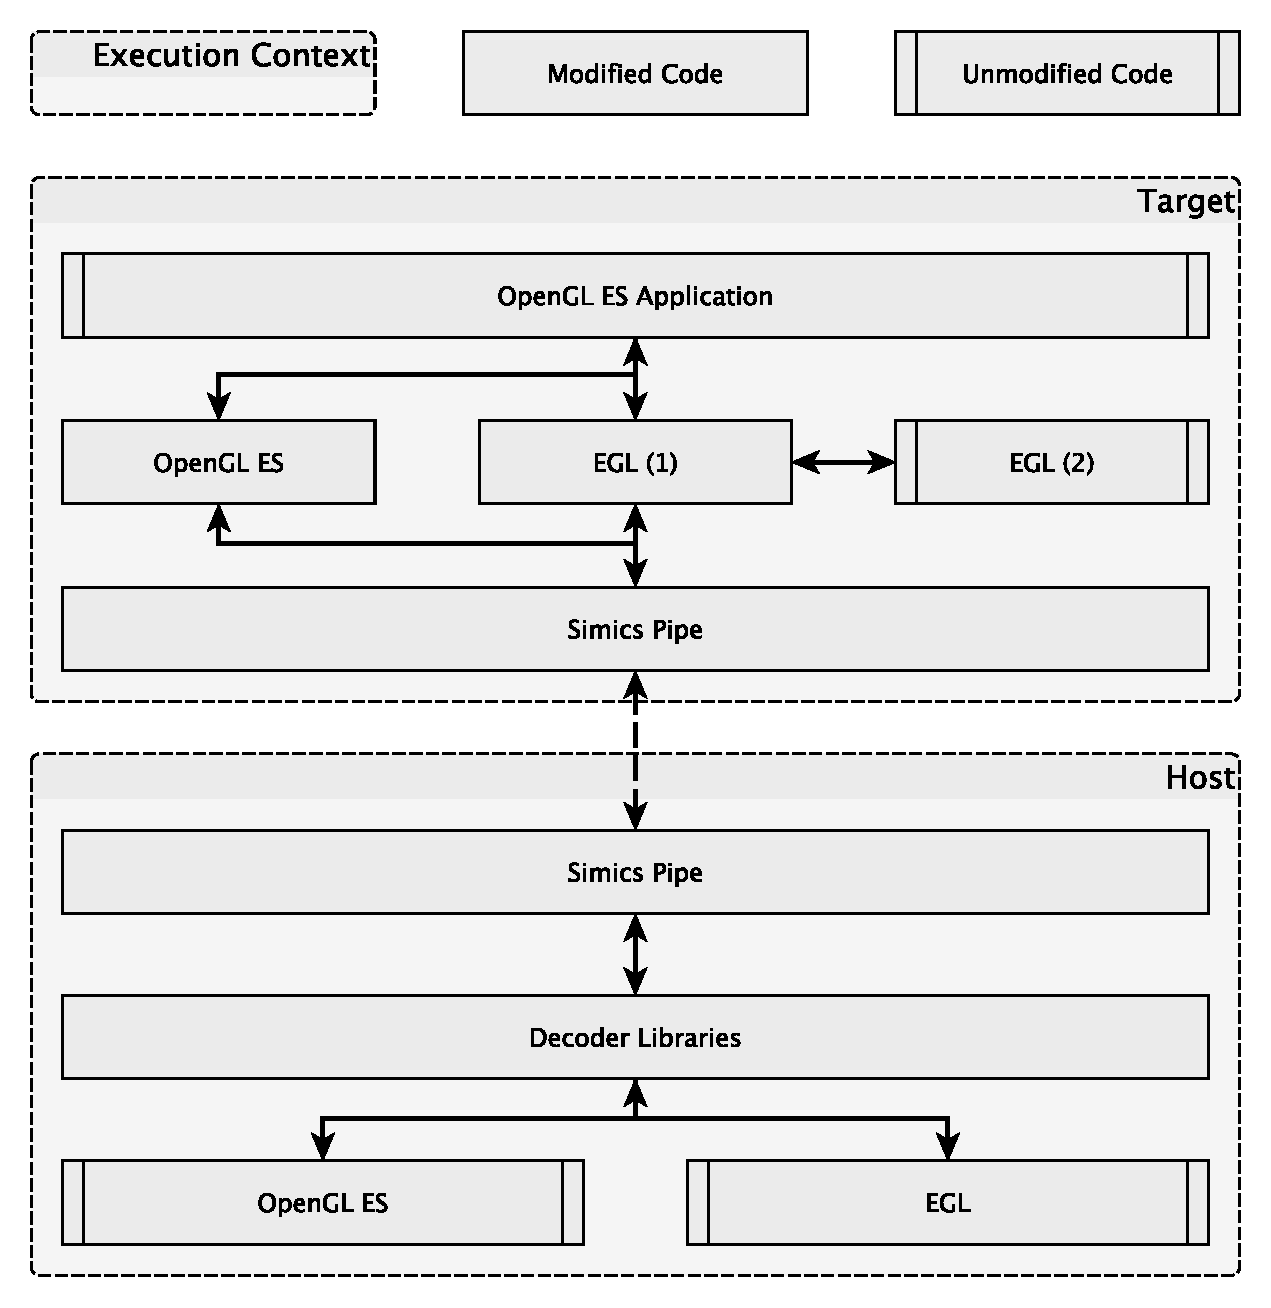
\includegraphics[height=0.7\textheight]{yedoverview.pdf}
  \end{center}

\end{columns}

\end{frame}


	\subsection{Simics pipe}
	\begin{frame}
\frametitle{Simics Pipe}

\begin{center}
	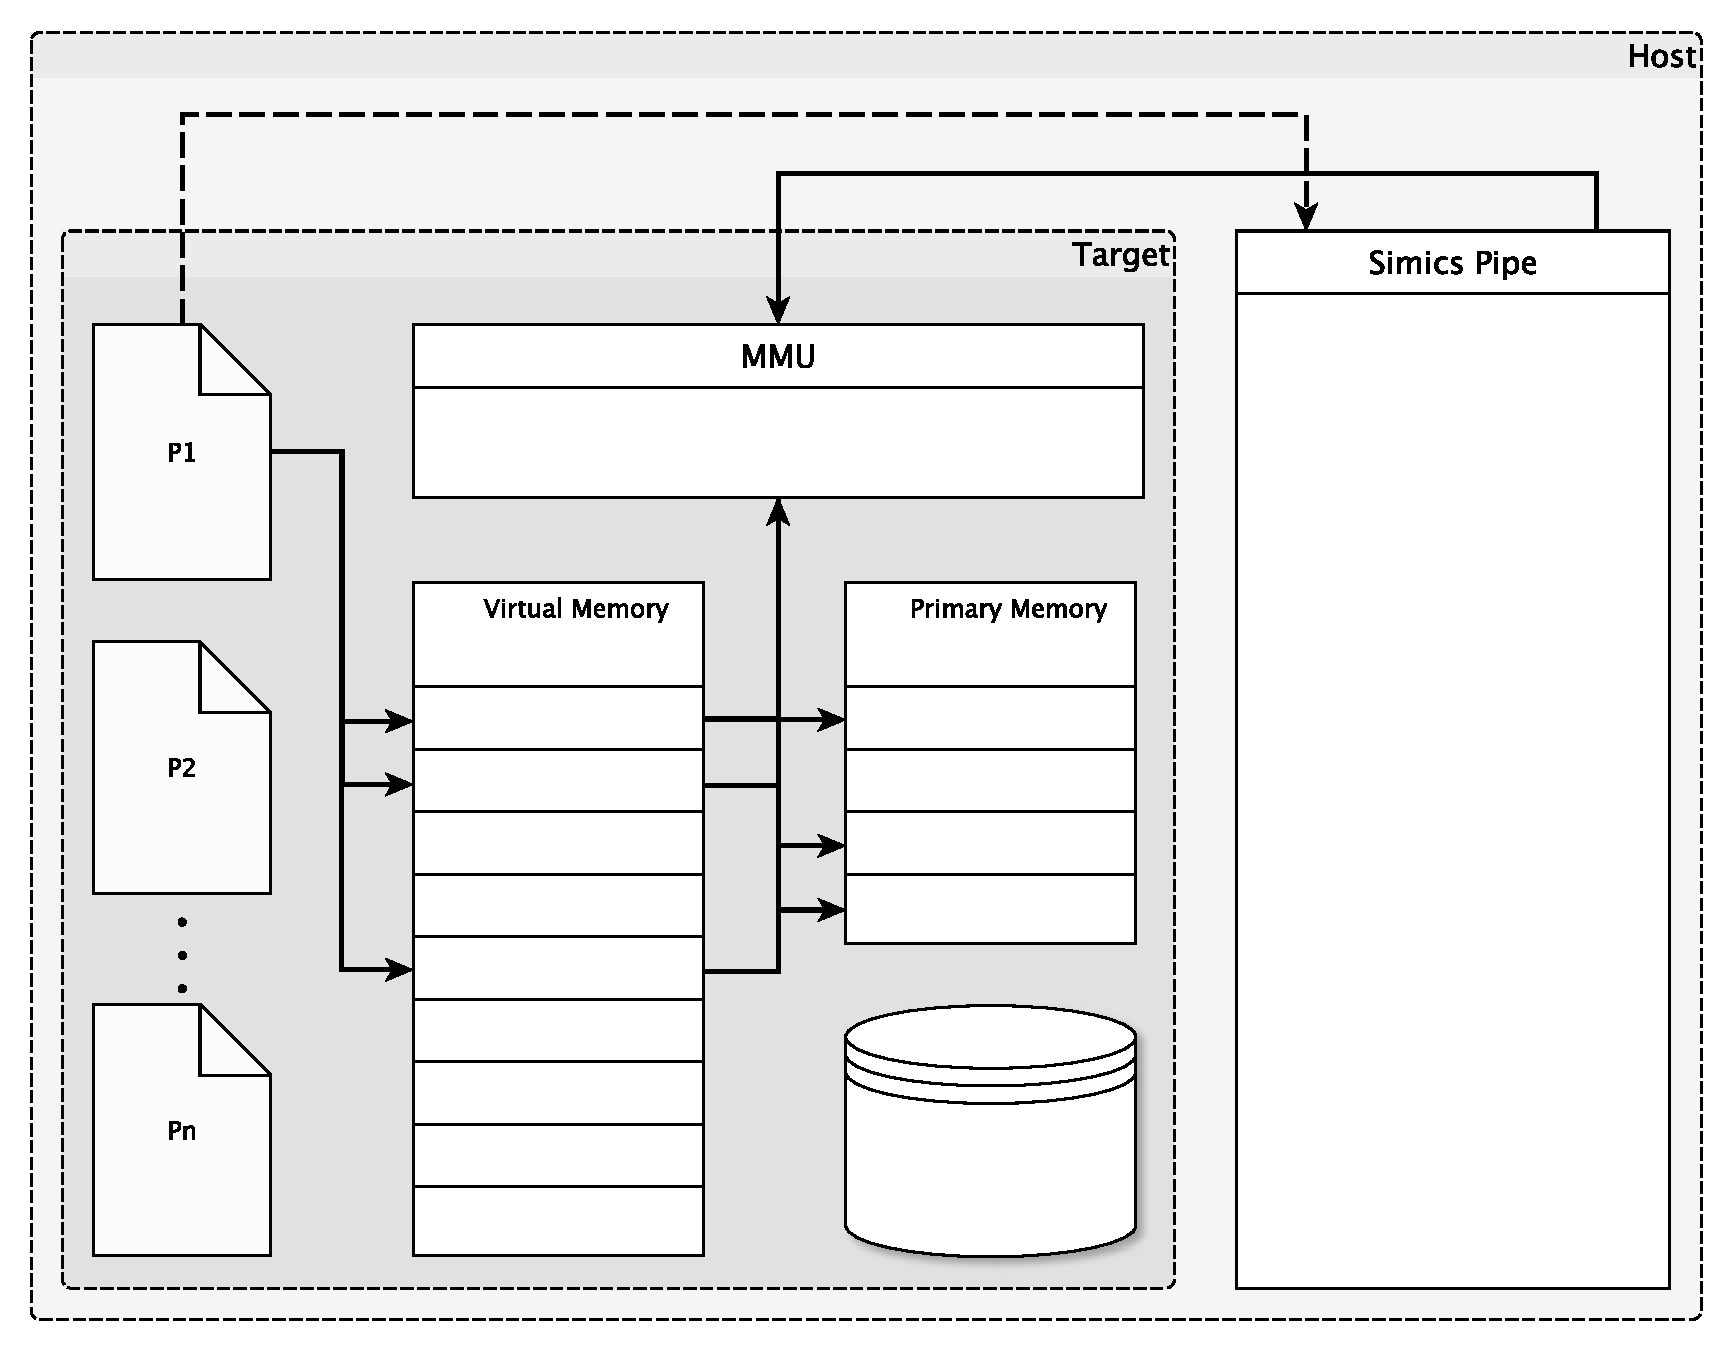
\includegraphics[height=0.8\textheight]{yedvirtualmemory.pdf}
\end{center}

\end{frame}

%% Memory translation overview. The OpenGL process hands a virtual memory
%% address, pointing somewhere in the target system \textit{primary}
%% memory, to the paravirtualized solution - which inquiries the target
%% system MMU to retrieve designated bytestream directly from target
%% physical memory.


        \subsection{Benchmarks}
	\begin{frame}[allowframebreaks]
\frametitle{Benchmarks}

%% % figbenchmarks.tex

\begin{figure}

\minipage{0.32\textwidth}
	
\includegraphics[width=\linewidth]{imgchess.png}
	\caption[Chess benchmark screen capture]{Chess.}
	\label{fig:benchmarks_chess}
\endminipage\hfill
\minipage{0.32\textwidth}
	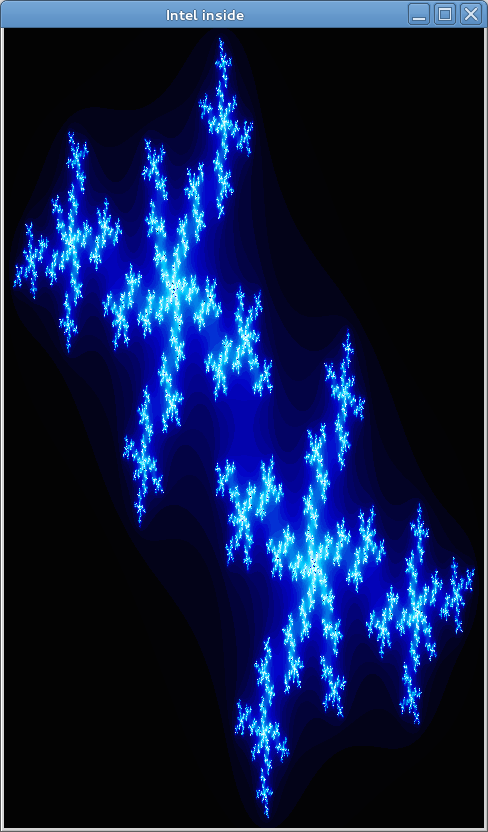
\includegraphics[width=\linewidth]{imgjulia.png}
	\caption[Julia benchmark screen capture]{Julia.}
	\label{fig:benchmarks_julia}
\endminipage\hfill
\minipage{0.32\textwidth}
  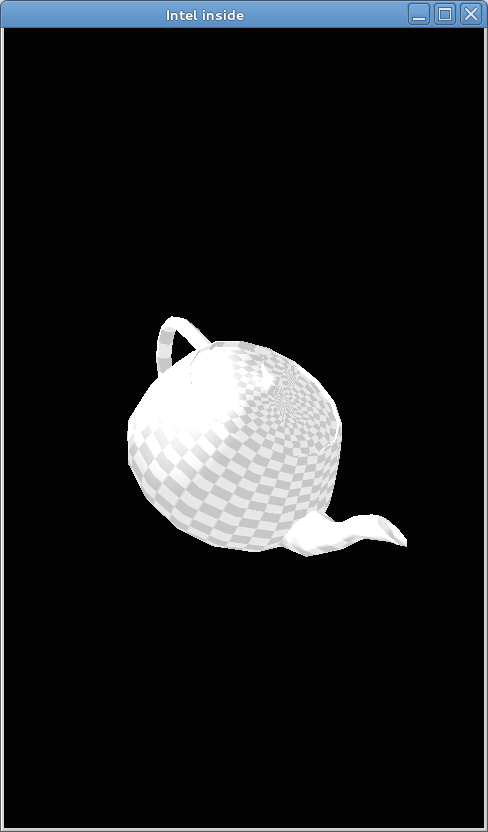
\includegraphics[width=\linewidth]{imgphong.png}
  \caption[Phong benchmark screen capture]{Phong.}
  \label{fig:benchmarks_phong}
\endminipage

\end{figure}

\framebreak 

%% \begin{block}{Input data variation}
%% \center
%% \resizebox{\linewidth}{!}{%
%% 	% tabkeyvals.tex

\begin{tabular}{lllll}
	Benchmark	& Input Data			& Halved Input		& Ref. Input		& Double Input		\\ \hline
	Chess		& No. Tiles				& $60\times60$		& $84\times84$		& $118\times118$	\\
	Julia		& No. Iterations		& $225$				& $450$				& $900$				\\
	Phong		& Texture Resolution	& $1448\times1448$	& $2048\times2048$	& $2896\times2896$	\\
\end{tabular}

%% }
%% \end{block}

%% \begin{block}{No. magic instructions}
%% \center
%% \resizebox{\linewidth}{!}{%
%% 	% tabkeyvalsmagicinstructions.tex

\begin{tabular}{lllll}
	Benchmark	& \phantom{Input Data}			& Halved Input	& Ref. Input	& Double Input	\\ \hline
	Chess		& \phantom{No. Tiles}			& $32403$		& $63507$		& $125319$		\\
	Julia		& \phantom{No. Iterations}		& $16$			& $16$			& $16$			\\
	Phong		& \phantom{Texture Resolution}	& $17$ 			& $17$ 			& $17$		\\
\end{tabular}

%% }
%% \end{block}
	
\end{frame}


        \subsection{Results}
        \begin{frame}
  \frametitle{Results - Chess}

  \begin{table}[]
    \centering
    \begin{tabular}{lllll}
      \hline
      Input & \multicolumn{4}{l}{Elapsed time (ms)} \\ \hline
      Tiles & Min & Max & Std & Avg \\
      $60\times60$ & \mascfirstline{simicschess60x60.dat.min} & \mascfirstline{simicschess60x60.dat.max} & \mascfirstline{simicschess60x60.dat.std} & \textbf{\mascfirstline{simicschess60x60.dat.avg}} \\
      $84\times84$ & \mascfirstline{simicschess84x84.dat.min} & \mascfirstline{simicschess84x84.dat.max} & \mascfirstline{simicschess84x84.dat.std} & \textbf{\mascfirstline{simicschess84x84.dat.avg}} \\
      $118\times118$ & \mascfirstline{simicschess118x118.dat.min} & \mascfirstline{simicschess118x118.dat.max} & \mascfirstline{simicschess118x118.dat.std} & \textbf{\mascfirstline{simicschess118x118.dat.avg}} \\ \hline
    \end{tabular}
    \caption{Software rasterization}
  \end{table}

  \begin{table}[]
    \centering
    \begin{tabular}{lllll}
      \hline
      Input & \multicolumn{4}{l}{Elapsed time (ms)} \\ \hline
      Tiles & Min & Max & Std & Avg \\
      $60\times60$ & \mascfirstline{parachess60x60.dat.min} & \mascfirstline{parachess60x60.dat.max} & \mascfirstline{parachess60x60.dat.std} & \textbf{\mascfirstline{parachess60x60.dat.avg}} \\
      $84\times84$ & \mascfirstline{parachess84x84.dat.min} & \mascfirstline{parachess84x84.dat.max} & \mascfirstline{parachess84x84.dat.std} & \textbf{\mascfirstline{parachess84x84.dat.avg}} \\
      $118\times118$ & \mascfirstline{parachess118x118.dat.min} & \mascfirstline{parachess118x118.dat.max} & \mascfirstline{parachess118x118.dat.std} & \textbf{\mascfirstline{parachess118x118.dat.avg}} \\ \hline
    \end{tabular}
    \caption{Paravirtualization}
  \end{table}

\end{frame}

    %% \begin{table}
    %%   \resizebox{0.95\columnwidth}{!}{%
    %%   \begin{tabular}{|c|c|r|r|r|r|}
    %%     \hline
    %%     \multirow{2}{*}{Benchmark} & \multirow{2}{*}{Input} & \multicolumn{4}{p{4cm}|}{\centering Elapsed time (\milli\second )} \\
    %%     \cline{3-6} && \multicolumn{1}{c|}{Min} & \multicolumn{1}{c|}{Max} & \multicolumn{1}{c|}{Std} & \multicolumn{1}{c|}{Avg} \\ \hline
    %%     \multirow{3}{*}{Chess} & \chesskeyone & \mascfirstline{parachess60x60.dat.min} & \mascfirstline{parachess60x60.dat.max} & \mascfirstline{parachess60x60.dat.std} & \textbf{\mascfirstline{parachess60x60.dat.avg}} \\
    %%     & \chesskeytwo & \mascfirstline{parachess84x84.dat.min} & \mascfirstline{parachess84x84.dat.max} & \mascfirstline{parachess84x84.dat.std} & \textbf{\mascfirstline{parachess84x84.dat.avg}} \\
    %%     & \chesskeythree & \mascfirstline{parachess118x118.dat.min} & \mascfirstline{parachess118x118.dat.max} & \mascfirstline{parachess118x118.dat.std} & \textbf{\mascfirstline{parachess118x118.dat.avg}} \\ \hline
    %%     \multirow{3}{*}{Julia} & \juliakeyone & \mascfirstline{parajulia225.dat.min} & \mascfirstline{parajulia225.dat.max}	& \mascfirstline{parajulia225.dat.std} & \textbf{\mascfirstline{parajulia225.dat.avg}} \\
    %%     & \juliakeytwo & \mascfirstline{parajulia450.dat.min} & \mascfirstline{parajulia450.dat.max} & \mascfirstline{parajulia450.dat.std} & \textbf{\mascfirstline{parajulia450.dat.avg}} \\
    %%     & \juliakeythree & \mascfirstline{parajulia900.dat.min} & \mascfirstline{parajulia900.dat.max} & \mascfirstline{parajulia900.dat.std} & \textbf{\mascfirstline{parajulia900.dat.avg}} \\ \hline
    %%   \end{tabular}
    %%   }
    %%   \caption{Paravirtualization}
    %% \end{table}

        % presentationresultsjulia.tex

\begin{frame}
\frametitle{Simics histograms: Julia}

\begin{center}
\resizebox{0.8\textwidth}{!}{%
	\input{gnuhistogramssimicsparajulia.tex}
}
\end{center}

\end{frame}

        \subsection{Hardware-assisted virtualization}
        \begin{frame}
\frametitle{\sout{Hardware-assisted virtualization}}

\begin{center}
Measurements collected without hardware-assisted virtualization:
\end{center}

\begin{table}[]
\centering
\caption{Chess}
\begin{tabular}{ll}
\hline
Paravirtualization & Software Rasterization \\ \hline
$\approx 1$ sec. & $\approx 7$ sec. \\
$\approx 2$ sec. & $\approx 10$ sec. \\
$\approx 3$ sec. & $\approx 13$ sec. \\ \hline
\end{tabular}
\end{table}

\begin{table}[]
\centering
\caption{Julia}
\begin{tabular}{lll}
\hline
Paravirtualization & Software Rasterization \\ \hline
$<\frac{1}{10}$ sec. & $\approx 1$ min. \\
$<\frac{1}{10}$ sec. & $<2$ min. \\
$\approx \frac{1}{10}$ sec. & $\approx 3$ min. \\ \hline
\end{tabular}
\end{table}

\end{frame}


        \section{Conclusion}

        \subsection{Future work}
	\begin{frame}

\frametitle{Future work}

\begin{itemize}
  \item Command serialization batching \begin{itemize}\item WireGL\end{itemize}
  \item Extending supported frameworks \begin{itemize}\item DirectX $\rightarrow$ OpenGL\end{itemize}
  \item General purpose, GPGPU \begin{itemize}\item OpenCL\end{itemize}
\end{itemize}

\end{frame}


        \subsection{Recap}
	\begin{frame}
\frametitle{Recap}

\begin{block}{\#1}
	Paravirtualization is a viable method of accelerating graphics
\end{block}

\begin{block}{\#2}
	Magic instructions is a suitable communications medium
\end{block}

\begin{block}{\#3}
	The case for paravirtualization is strengthened for systems where hardware-assisted virtualization is unavailable
\end{block}

\end{frame}


        \begin{frame}

\begin{center}
\url{http://www.windriver.com/products/simics/}
\end{center}

\end{frame}


        % Appendix
        \begin{frame}
  \frametitle{Histograms}

  \begin{columns}[t]

    \column{0.4\textwidth}

    Chess
    \begin{itemize}
    \item Magic instruction overhead could account for majority of elapsed frame time
    \end{itemize}

    Julia
    \begin{itemize}
    \item Two to three peaks in sample distribution
    \item Unclear why
    \end{itemize}

    \column{0.7\textwidth}

    \resizebox{\textwidth}{!}{%
      \input{gnuhistogramssimicsparachess.tex}
    }

    \vspace{.5cm}

    \resizebox{\textwidth}{!}{%
      \input{gnuhistogramssimicsparajulia.tex}
    }

  \end{columns}

\end{frame}

\end{document}
